\documentclass[a4paper,12pt]{article}
\usepackage{graphicx}
\usepackage{geometry}
\usepackage{amsmath}
\usepackage{listings}
\usepackage{hyperref}
\usepackage{titlesec}
\usepackage{fancyhdr}
\usepackage{booktabs}
\usepackage{xcolor}

% Define color for code
\definecolor{codecolor}{rgb}{0.0,0.0,0.6}

% Page setup
\geometry{margin=1in}

% Formatting section titles
\titleformat{\section}{\large\bfseries}{\thesection}{1em}{}
\titleformat{\subsection}{\normalsize\bfseries}{\thesubsection}{1em}{}

% Header and footer
\pagestyle{fancy}
\fancyhf{}
\fancyhead[L]{\textbf{Arduino-Based Digital Clock}}
\fancyfoot[C]{\thepage}
\renewcommand{\headrulewidth}{0.4pt}

% Custom listing style for Arduino code
\lstdefinestyle{arduinoStyle}{
    language=C,
    basicstyle=\ttfamily\footnotesize\color{codecolor},
    keywordstyle=\color{blue}\bfseries,
    commentstyle=\color{green!60!black}\itshape,
    stringstyle=\color{red},
    numbers=left,
    numberstyle=\tiny\color{gray},
    stepnumber=1,
    numbersep=5pt,
    backgroundcolor=\color{gray!10},
    showspaces=false,
    showstringspaces=false,
    showtabs=false,
    frame=single,
    tabsize=2,
    captionpos=b,
    breaklines=true,
    breakatwhitespace=false
}

% Title and Author
\title{\textbf{Arduino-Based Digital Clock Using Seven-Segment Displays and 7447 Decoder}}
\author{Niketh Achanta - EE24BTECH11047}
\date{}

\begin{document}

\maketitle

\begin{abstract}
This report presents the design and implementation of an Arduino-based digital clock using six seven-segment displays and a 7447 BCD-to-seven-segment decoder. The clock functions using multiplexing to efficiently control the displays and maintain accurate timekeeping without using an external RTC module.
\end{abstract}

\section{Introduction}
Digital clocks are an essential part of embedded systems and electronic circuits. This project aims to design a functional digital clock using an \textbf{Arduino}, \textbf{six seven-segment displays}, and a \textbf{7447 BCD-to-seven-segment decoder}. The clock displays hours, minutes, and seconds while ensuring efficient power usage and reducing the number of I/O pins required. Instead of directly controlling all six displays, multiplexing is used to rapidly switch between them.

\section{Components Used}
The main components required for this project are listed in Table \ref{tab:components}.

\begin{table}[h]
    \centering
    \renewcommand{\arraystretch}{1.2}
    \begin{tabular}{ll}
        \toprule
        \textbf{Component} & \textbf{Description} \\
        \midrule
        Arduino Uno & Microcontroller used for controlling the clock \\
        6x Seven-Segment Display & Displays hours, minutes, and seconds \\
        7447 BCD to 7-Segment Decoder & Converts BCD values to 7-segment signals \\
        Resistors (220$\Omega$) & Current limiting resistors for display protection \\
        Wires \& Breadboard & Circuit assembly and connections \\
        \bottomrule
    \end{tabular}
    \caption{Components used in the project}
    \label{tab:components}
\end{table}

\section{Multiplexing Concept}
Since an Arduino does not have enough I/O pins to control all six displays independently, \textbf{multiplexing} is used. This technique involves activating one display at a time while rapidly cycling through all six, creating the illusion of a continuous display due to \textbf{persistence of vision}.

\subsection{How Multiplexing Works}
\begin{itemize}
    \item The Arduino outputs a \textbf{BCD} value corresponding to each digit.
    \item The 7447 decoder converts BCD to the seven-segment format.
    \item Control signals determine which display is active at any given moment.
    \item The Arduino cycles through all six displays multiple times per second.
    \item Each display is active for a short period (typically 5ms).
    \item At a refresh rate above 60Hz (entire cycle less than 16.7ms), no flickering is visible.
\end{itemize}

\section{Circuit Diagram}
Figure \ref{fig:7seg} illustrates the seven-segment display pin configuration, and Figure \ref{fig:7447} shows the 7447 BCD decoder.

\begin{figure}[h]
    \centering
    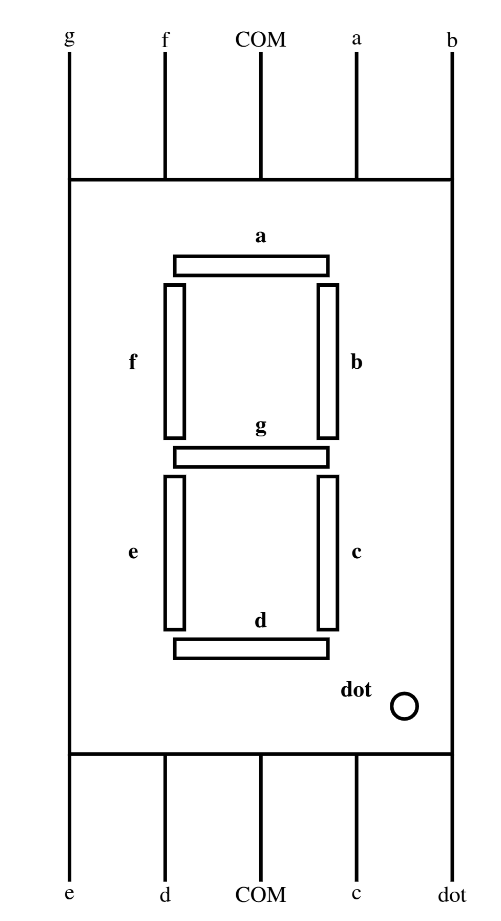
\includegraphics[width=0.5\textwidth]{figs\image.png}
    \caption{Common Cathode Seven-Segment Display Pinout}
    \label{fig:7seg}
\end{figure}

\begin{figure}[h]
    \centering
    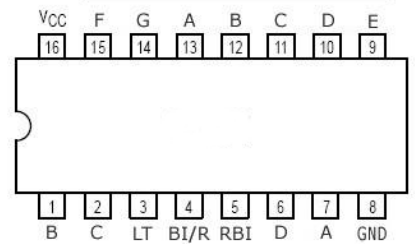
\includegraphics[width=0.6\textwidth]{figs\image1.png}
    \caption{7447 BCD-to-Seven-Segment Decoder Pinout}
    \label{fig:7447}
\end{figure}

\section{Pinout diagrams}
The circuit consists of three main elements:

\subsection{Display Circuit}
Each seven-segment display is connected to the 7447 decoder through current-limiting resistors. The common cathode of each display is connected to ground through a transistor that acts as a switch.

\subsection{Decoder Circuit}
The 7447 decoder receives 4-bit BCD inputs from the Arduino and converts them to the appropriate seven-segment patterns. All six displays share the same decoder outputs, but only one display is active at any given time.

\subsection{Control Circuit}
The Arduino controls which display is active by turning on the corresponding transistor. Six output pins (PD6, PD7, PB0, PB1, PB2, PB3) are used to select which display is active, while four pins (PD2, PD3, PD4, PD5) provide the BCD data.

\section{Code Implementation}
The Arduino code is structured as follows:
\begin{itemize}
    \item Initializes all required pins for \textbf{BCD input} and \textbf{display control}.
    \item Uses a \textbf{timer interrupt} to increment the clock every second.
    \item Implements \textbf{multiplexing} to update the display efficiently.
\end{itemize}


\subsection{Code Explanation}
\subsubsection{BCD Time Representation}
Time values are stored in Binary-Coded Decimal (BCD) format, where each decimal digit is represented by its 4-bit binary equivalent. For example, 12:34:56 is stored as:

\begin{itemize}
    \item hours = 0001 0010 (0x12)
    \item minutes = 0011 0100 (0x34)
    \item seconds = 0101 0110 (0x56)
\end{itemize}

\subsubsection{Timer Configuration}
The timer is configured to generate an interrupt every second:

\begin{itemize}
    \item Timer1 operates in CTC (Clear Timer on Compare) mode
    \item With a 16MHz clock and 1024 prescaler, Timer1 increments at 15,625Hz
    \item The compare match value (OCR1A) is set to 15,624, resulting in an interrupt frequency of 1Hz
\end{itemize}

\subsubsection{Multiplexing Implementation}
The displayTime() function implements multiplexing by:

\begin{enumerate}
    \item Extracting individual digits from the BCD time variables
    \item Activating one display at a time using its control pin
    \item Setting the BCD output pins to show the correct digit
    \item Keeping each display on for 5ms before moving to the next
    \item Cycling through all six displays continuously
\end{enumerate}

\section{Conclusion}
This project successfully implemented a digital clock using an Arduino, multiplexed seven-segment displays, and a 7447 decoder. The multiplexing approach significantly reduces the required I/O pins while maintaining accurate timekeeping. The design uses timer interrupts for precise one-second timing and efficiently manages six displays using just ten output pins from the Arduino.

The implementation demonstrates fundamental concepts in digital electronics including:
\begin{itemize}
    \item Multiplexing techniques for display control
    \item BCD to seven-segment conversion
    \item Timer configuration for precise timing
    \item Interrupt-based timekeeping
\end{itemize}

\end{document}

